\section{Understanding \S~138 of the Negotiable Instruments Act} \label{app:understanding}

As per \S~138 of the Negotiable Instruments Act, 1881, if a cheque (drawn by a person for paying off a debt or a liability) is returned unpaid due to insufficiency of funds or credit, the payer may be imprisoned for up to two years or with a fine up to twice the amount of the cheque, or both.\footcite[A \textit{cheque} is defined as per \S~6 of the NI Act. It is a bill of exchange drawn on a specified banker and not expressed to be payable otherwise than on-demand. It includes the electronic image of a truncated cheque and a cheque in electronic form. Once a cheque has been signed and issued in favour of the holder of the cheque, there is a statutory presumption \S~139 of NI Act that the cheque is issued in discharge of a legally enforceable debt or liability. However, said presumption is a rebuttable one. The issuer of the cheque can rebut that presumption by adducing credible evidence that the cheque was issued for some other purpose like security for a loan.][]{sc2018_murugun} However, this is only the case when: (i) the payee presents the cheque within six months of its issuance, (ii) demand for the payment within thirty days of the return of the cheque by the bank, and (iii) the payer fails to pay within fifteen days of the receipt of such notice. The cause of action arises after these fifteen days. The payee subsequently has one month to file a complaint before the appropriate court.

An offence within the contemplation of \S~138 is complete with the dishonour of the cheque, but taking cognisance of the same by any court is forbidden so long as the complainant does not have the cause of action to file a complaint.\footcite{sc2014_dashrath} This is because the legislature has considered it appropriate to allow the drawer of a dishonoured cheque to pay up the amount before permitting her prosecution. The accused has a right to pay the money within fifteen days from the date of the service of notice, and only when she fails to pay is it open for the complainant to file a complaint. Thus, in \citetitle{sc2002_shakti}, where a complaint failed to mention that notice had been served, the same was not maintainable.\footcite{sc2002_shakti}

A complainant may approach the concerned court within one month of the time provided to the payer to satisfy his debt or liability. After an amendment in 2015, the Act has been modified to prescribe that the territorial jurisdiction for filing of a cheque dishonour complaint shall be restricted to the court within whose territorial jurisdiction the offence is committed, i.e., which is the location where the cheque is dishonoured or returned unpaid by the bank on which it is drawn. Place of issuance or delivery of the statutory notice or where the complainant chooses to present the cheque for encashment by his bank is relevant for determining territorial jurisdiction for filing cheque dishonour complaints.

Once a complaint is led in court, the court takes cognisance and issues the process for producing the accused. If the accused fails to appear, the court may issue a suitable warrant to ensure the same. As per \S~143 of the Act, cases are meant to be tried summarily. However, if the court believes that the nature of the matter is such that a sentence of imprisonment for a term exceeding one year may have to be passed or that it is, for any other reason, undesirable to try the case summarily, it may record such an order and hear the cases as a summons trial.\footnote{In case of a summary trial, if the accused pleads not guilty, the magistrate may record the substance of the evidence and deliver a judgment. However, in a summons trial, the proceeding is as any ordinary matter followed by a judgment.}

Notably, the Supreme Court has observed that for the offence \S~138, the compensatory aspect of the remedy should be prioritised over the punitive aspect.\footcite{sc2010_damodar} Waiver of imprisonment instead of payment of additional compensation is permissible under exceptional circumstances.\footcite{sc2018_priyanka} The court may close proceedings if the accused deposits the amount assessed by it regarding the cheque amount, interest/costs, etc., within the stipulated period. Compounding at the initial stage and even at a later stage is acceptable.\footcite{sc2018_meters} 

For brevity, \cref{fig:proceeding_138} demonstrates the course of a proceeding in the case of a cheque dishonour.

\begin{figure}
\caption{Proceeding \S~138 of the Negotiable Instruments Act}
\label{fig:proceeding_138}
\vspace*{0.5cm}
\centering 
\begin{tikzpicture}[node distance= 1cm, text width=2.5cm]
\node (in0) [note] {};
\node (in1) [main, fill=red!30, below = 0.5cm of in0, yshift = 0.8cm] {Dishonour};
\node (in2) [process, below = 0.5cm of in1] {Demand payment};
\node (in3) [process, below = 0.5cm of in2, xshift = -3cm] {Does not pay};
\node (in4) [main, fill=red!30, below = 0.5cm of in2, xshift = 3cm] {Pays};
\node (in5) [process, below = 0.5cm of in3]{Court proceedings};
\node (in6) [process, below = 0.5cm of in5, xshift = -3cm] {Accused not present};
\node (in7) [process, below = 0.5cm of in6] {Warrant};
\node (in8) [process, below = 1.9cm of in5, xshift = 3cm] {Present};
\node (in9) [process, below = 0.5cm of in8, xshift = -3cm] {Summary proceeding};
\node (in10) [process, below = 0.5cm of in8, xshift = 3cm] {Summons proceeding};
\node (in11) [process, below = 0.5cm of in10] {Trial};
\node (in12) [main, fill=red!30, below = 0.5cm of in11] {Judgement};

\draw [arrow] (in1) -- (in2);
\draw [arrow] (in2) -| (in3);
\draw [arrow] (in2) -| (in4);
\draw [arrow] (in3) -- (in5);
\draw [arrow] (in5) -| (in6);
\draw [arrow] (in5) -| (in8);
\draw [arrow] (in6) -- (in7);
\draw [arrow] (in7) -- (in8);
\draw [arrow] (in8) |- (in9);
\draw [arrow] (in8) |- (in10);
\draw [arrow] (in10) -- (in11);
\draw [arrow] (in11) -- (in12);
\draw [arrow] (in9) |- (in12);

\end{tikzpicture}
\end{figure}

\pagebreak

\section{Criteria for sample selection} \label{sec:sample_selection}

\textcolor{red}{Manish, please populate the table below.}

\begin{longtable}{p{0.32\textwidth}p{0.6\textwidth}}
\label{tab:sample_selection}
\\
\toprule
\multicolumn{2}{c}{\textbf{States Excluded}} \\ \midrule
\multicolumn{1}{c|}{\textbf{Criteria}} & \multicolumn{1}{c}{\textbf{States}} \\ \midrule
\multicolumn{1}{p{0.32\textwidth}|}{Unable to download sample data} & \\ \midrule
\multicolumn{1}{p{0.32\textwidth}|}{No cases related to \gls{ni}} & \\ \midrule
\multicolumn{1}{p{0.32\textwidth}|}{\textless 2\% of the final orders are machine-readable and in English} & \\ \midrule
\multicolumn{2}{c}{\textbf{Final Sample}} \\ \midrule
 \multicolumn{2}{p{0.92\textwidth}}{\textit{Andhra Pradesh, Chandigarh, Delhi, Goa, Gujarat, Haryana, Himachal Pradesh, Karnataka, Maharashtra, and Punjab.}} \\ \bottomrule
\end{longtable}

\pagebreak

\section{Robustness checks}\label{sec:robustness}
In this section we describe the robustness checks we performed to assess how confident we can be in the results of the fixed-effects model.

\subsection{Consistency}
\label{sec:consistency}
As Tables \ref{tab:yearFE}, \ref{tab:hearFE}, \ref{tab:durationStateWise}, \ref{tab:hearingsStateWise} show, the year of filing and the state both have a significant effect on the duration of the case and the number of hearings required to dispose it. This supports our decision to control for state and year fixed effects in our main analysis.

{\footnotesize \begin{longtable}{lcc|ccc} 
 \caption{Disposal Days: Variation across years}\label{tab:yearFE}
 \\[-1.8ex]
 \hline \\[-1.8ex] 
 & \multicolumn{5}{c}{\textit{Dependent variable: Disposal days}} \\ 
 \cline{2-6} 
 \\[-1.8ex] & (2014) & (2015) & (2016) & (2017) & (2018)\\ 
 \hline \\[-1.8ex]
 
 D(non-Appearance) & 155.424$^{***}$ & 186.156$^{***}$ & 220.051$^{***}$ & 185.167$^{***}$ & 242.311$^{***}$ \\ 
 & (8.163) & (8.921) & (10.899) & (13.316) & (14.042) \\ 
 & & & & & \\ 
 D(Summons) & 35.087$^{***}$ & 29.933$^{***}$ & 118.444$^{***}$ & 182.578$^{***}$ & 220.014$^{***}$ \\ 
 & (8.335) & (8.710) & (11.340) & (14.351) & (17.025) \\ 
 & & & & & \\ 
 D(Mediation) & 61.687$^{***}$ & 37.802$^{***}$ & 76.600$^{***}$ & 156.578$^{***}$ & 255.746$^{***}$ \\ 
 & (7.862) & (8.316) & (10.465) & (13.797) & (17.196) \\ 
 & & & & & \\ 
 D(Jurisdiction) & 180.482$^{***}$ & 231.023$^{***}$ & 269.201$^{***}$ & 313.779$^{***}$ & 318.416$^{***}$ \\ 
 & (9.022) & (8.876) & (10.238) & (12.909) & (13.564) \\ 
 & & & & & \\ 
 D(Multiplicity) & 64.826$^{***}$ & 138.977$^{***}$ & 141.382$^{***}$ & 201.150$^{***}$ & 246.812$^{***}$ \\ 
 & (19.158) & (17.088) & (20.037) & (24.870) & (31.392) \\ 
 & & & & & \\ 
 D(Contested) & 5.510 & $-$12.717 & $-$59.490$^{***}$ & $-$75.624$^{***}$ & $-$71.797$^{***}$ \\ 
 & (10.927) & (10.419) & (11.695) & (12.818) & (13.581) \\

 \hline \\[-1.8ex]
 State FE & Y & Y & Y & Y & Y \\
 \hline \\[-1.8ex] 
 
 Observations & 6,760 & 8,458 & 8,165 & 6,117 & 5,927 \\ 
 R$^{2}$ & 0.189 & 0.202 & 0.228 & 0.232 & 0.269 \\ 
 Adjusted R$^{2}$ & 0.187 & 0.201 & 0.226 & 0.230 & 0.268 \\
 
 \hline \\[-1.8ex] 
 \multicolumn{6}{l}{\textit{Note:} $^{*}$p$<$0.1; $^{**}$p$<$0.05; $^{***}$p$<$0.01} \\
\end{longtable}
}
\pagebreak

{\footnotesize \begin{longtable}{lcc|ccc} 
 \caption{Number of hearings: Variation across years}\label{tab:hearFE} 
 \\[-1.8ex] 
 \hline \\[-1.8ex] 
 & \multicolumn{5}{c}{\textit{Dependent variable: Number of hearings}} \\ 
 \cline{2-6} 
 \\[-1.8ex] & 2014 & 2015 & 2016 & 2017 & 2018 \\ 
 \hline \\[-1.8ex] 
 D(non-Appearance) & 5.996$^{***}$ & 6.809$^{***}$ & 6.929$^{***}$ & 7.764$^{***}$ & 8.049$^{***}$ \\ 
 & (0.221) & (0.236) & (0.279) & (0.362) & (0.364) \\ 
 & & & & & \\ 
 D(Summons) & 3.773$^{***}$ & 5.041$^{***}$ & 7.678$^{***}$ & 10.391$^{***}$ & 11.416$^{***}$ \\ 
 & (0.226) & (0.231) & (0.290) & (0.390) & (0.442) \\ 
 & & & & & \\ 
 D(Mediation) & 1.967$^{***}$ & 1.653$^{***}$ & 2.828$^{***}$ & 4.868$^{***}$ & 7.090$^{***}$ \\ 
 & (0.213) & (0.220) & (0.267) & (0.375) & (0.446) \\ 
 & & & & & \\ 
 D(Jurisdiction) & 2.973$^{***}$ & 4.911$^{***}$ & 5.133$^{***}$ & 7.023$^{***}$ & 6.345$^{***}$ \\ 
 & (0.244) & (0.235) & (0.262) & (0.350) & (0.352) \\ 
 & & & & & \\ 
 D(Multiplicity) & 5.756$^{***}$ & 8.732$^{***}$ & 9.122$^{***}$ & 10.539$^{***}$ & 12.298$^{***}$ \\ 
 & (0.518) & (0.452) & (0.512) & (0.675) & (0.815) \\ 
 & & & & & \\ 
 D(Contested) & 5.157$^{***}$ & 4.213$^{***}$ & 3.139$^{***}$ & 2.230$^{***}$ & 1.341$^{***}$ \\ 
 & (0.296) & (0.276) & (0.299) & (0.348) & (0.352) \\ 
 \hline \\[-1.8ex]
 State FE & Y & Y & Y & Y & Y \\
 \hline \\[-1.8ex] 
 Observations & 6,760 & 8,458 & 8,165 & 6,117 & 5,927 \\ 
 R$^{2}$ & 0.317 & 0.348 & 0.372 & 0.384 & 0.389 \\ 
 Adjusted R$^{2}$ & 0.316 & 0.346 & 0.370 & 0.382 & 0.388 \\ 
 \hline \\[-1.8ex] 
 \multicolumn{6}{l}{\textit{Note:} $^{*}$p$<$0.1; $^{**}$p$<$0.05; $^{***}$p$<$0.01} \\ 
 \end{longtable}
} 
 \begin{landscape}
 \pagestyle{empty}
 \begin{table}
 \centering
 \caption{Disposal Days: Variation across States}\label{tab:durationStateWise}
 \scalebox{0.75}{
 \hspace*{-0.7cm}
 \begin{tabular}{lcccccccccc} 
 \\[-1.8ex]
 \hline \\[-1.8ex] 
 & \multicolumn{10}{c}{\textit{Dependent variable: Disposal days}} \\ 
 \cline{2-11} 
 & (Punjab) & (Maharashtra) & (Karnataka) & (Himachal Pradesh) & (Haryana) & (Gujarat) & (Goa) & (Delhi) & (Chandigarh) & (Andhra Pradesh) \\ 
 \hline \\[-1.8ex] 
 D(non-Appearance) & 282.470$^{***}$ & 117.295$^{***}$ & 219.113$^{***}$ & 217.113$^{***}$ & 231.698$^{***}$ & 193.737$^{***}$ & 261.782$^{***}$ & 227.051$^{***}$ & 329.881$^{***}$ & 152.268$^{***}$ \\ 
 & (45.895) & (12.643) & (8.354) & (40.559) & (37.703) & (12.871) & (98.140) & (13.886) & (55.699) & (17.760) \\ 
 & & & & & & & & & & \\ 
 D(Summons) & 134.133$^{***}$ & 107.435$^{***}$ & 43.375$^{***}$ & 153.415$^{***}$ & 155.525$^{***}$ & 388.108$^{***}$ & 361.641$^{***}$ & $-$17.411 & 86.252$^{***}$ & 169.039$^{***}$ \\ 
 & (10.040) & (19.458) & (11.362) & (40.332) & (11.272) & (26.752) & (59.235) & (14.558) & (20.949) & (21.555) \\ 
 & & & & & & & & & & \\ 
 D(Mediation) & 85.850$^{***}$ & 132.560$^{***}$ & 213.240$^{***}$ & 173.916$^{***}$ & 52.617$^{***}$ & 15.695 & 126.867$^{***}$ & $-$32.710$^{**}$ & 49.678$^{**}$ & 29.968 \\ 
 & (10.097) & (13.157) & (10.996) & (36.869) & (11.094) & (20.682) & (48.674) & (15.447) & (22.164) & (27.086) \\ 
 & & & & & & & & & & \\ 
 D(Jurisdiction) & 203.741$^{***}$ & 320.802$^{***}$ & 263.146$^{***}$ & 238.843$^{***}$ & 223.542$^{***}$ & 347.000$^{***}$ & 221.767$^{**}$ & 253.748$^{***}$ & 172.153$^{***}$ & 202.846$^{***}$ \\ 
 & (9.841) & (13.000) & (14.634) & (46.625) & (10.874) & (11.812) & (101.778) & (15.816) & (20.591) & (33.936) \\ 
 & & & & & & & & & & \\ 
 D(Multiplicity) & 146.651$^{***}$ & 293.331$^{***}$ & 230.515$^{***}$ & 99.971 & 93.660$^{***}$ & 18.436 & 162.484$^{*}$ & 101.022$^{***}$ & 156.640$^{***}$ & 160.606$^{***}$ \\ 
 & (20.751) & (42.522) & (21.832) & (92.582) & (17.977) & (43.271) & (96.128) & (32.579) & (40.015) & (37.491) \\ 
 & & & & & & & & & & \\ 
 D(Contested) & 87.051$^{***}$ & $-$155.963$^{***}$ & $-$44.687$^{***}$ & $-$23.156 & 86.789$^{***}$ & $-$104.434$^{***}$ & $-$162.420$^{***}$ & $-$120.015$^{***}$ & 9.070 & $-$104.016$^{***}$ \\ 
 & (17.045) & (15.169) & (8.636) & (52.987) & (16.530) & (17.941) & (54.347) & (21.355) & (31.604) & (20.176) \\
 \hline \\[-1.8ex]
 Year FE & Y & Y & Y & Y & Y & Y & Y & Y & Y & Y \\
 \hline \\[-1.8ex] 
 Observations & 4,949 & 4,930 & 9,017 & 640 & 4,130 & 4,881 & 274 & 3,824 & 686 & 2,096 \\ 
 R$^{2}$ & 0.214 & 0.245 & 0.246 & 0.259 & 0.209 & 0.301 & 0.260 & 0.259 & 0.251 & 0.149 \\ 
 Adjusted R$^{2}$ & 0.213 & 0.243 & 0.245 & 0.248 & 0.207 & 0.300 & 0.232 & 0.257 & 0.240 & 0.145 \\ 
 \hline \\[-1.8ex] 
 \multicolumn{11}{l}{\textit{Note:} $^{*}$p$<$0.1; $^{**}$p$<$0.05; $^{***}$p$<$0.01} \\ 
 \end{tabular}}
 \end{table}
 \end{landscape}

 \begin{landscape}
 \pagestyle{empty}
 \begin{table}
 \centering
 \caption{Number of hearings: Variation across States}\label{tab:hearingsStateWise}
 \scalebox{0.75}{
 \begin{tabular}{lcccccccccc} 
 \\[-1.8ex]
 \hline \\[-1.8ex] 
 & \multicolumn{10}{c}{\textit{Dependent variable: Number of hearings}} \\ 
 \cline{2-11}
 & (Punjab) & (Maharashtra) & (Karnataka) & (Himachal Pradesh) & (Haryana) & (Gujarat) & (Goa) & (Delhi) & (Chandigarh) & (Andhra Pradesh) \\ 
\hline \\[-1.8ex] 
 D(non-Appearance) & 7.600$^{***}$ & 7.560$^{***}$ & 7.425$^{***}$ & 5.558$^{***}$ & 4.860$^{***}$ & 5.241$^{***}$ & 6.959$^{**}$ & 3.628$^{***}$ & 8.292$^{***}$ & 7.522$^{***}$ \\ 
 & (1.329) & (0.329) & (0.220) & (0.654) & (0.966) & (0.339) & (2.955) & (0.174) & (1.501) & (0.628) \\ 
 & & & & & & & & & & \\ 
 D(Summons) & 5.428$^{***}$ & 8.064$^{***}$ & 7.352$^{***}$ & 4.930$^{***}$ & 5.504$^{***}$ & 17.208$^{***}$ & 14.333$^{***}$ & 1.858$^{***}$ & 4.982$^{***}$ & 18.646$^{***}$ \\ 
 & (0.291) & (0.506) & (0.299) & (0.650) & (0.289) & (0.704) & (1.784) & (0.182) & (0.564) & (0.762) \\ 
 & & & & & & & & & & \\ 
 D(Mediation) & 3.415$^{***}$ & 3.068$^{***}$ & 6.631$^{***}$ & 3.598$^{***}$ & 2.316$^{***}$ & 0.452 & 5.820$^{***}$ & 0.955$^{***}$ & 1.678$^{***}$ & 2.993$^{***}$ \\ 
 & (0.292) & (0.342) & (0.290) & (0.594) & (0.284) & (0.544) & (1.466) & (0.193) & (0.597) & (0.957) \\ 
 & & & & & & & & & & \\ 
 D(Jurisdiction) & 4.860$^{***}$ & 7.433$^{***}$ & 3.650$^{***}$ & 4.484$^{***}$ & 4.575$^{***}$ & 7.689$^{***}$ & 6.092$^{**}$ & 2.461$^{***}$ & 2.893$^{***}$ & 7.414$^{***}$ \\ 
 & (0.285) & (0.338) & (0.386) & (0.751) & (0.279) & (0.311) & (3.065) & (0.198) & (0.555) & (1.199) \\ 
 & & & & & & & & & & \\ 
 D(Multiplicity) & 8.708$^{***}$ & 12.314$^{***}$ & 14.762$^{***}$ & 2.704$^{*}$ & 5.261$^{***}$ & $-$0.259 & 9.605$^{***}$ & 5.538$^{***}$ & 10.163$^{***}$ & 10.706$^{***}$ \\ 
 & (0.601) & (1.106) & (0.575) & (1.492) & (0.460) & (1.139) & (2.895) & (0.407) & (1.078) & (1.325) \\ 
 & & & & & & & & & & \\ 
 D(Contested) & 10.062$^{***}$ & $-$1.049$^{***}$ & 1.758$^{***}$ & 2.959$^{***}$ & 8.682$^{***}$ & 0.513 & $-$0.066 & 0.466$^{*}$ & 4.183$^{***}$ & 0.958 \\ 
 & (0.493) & (0.395) & (0.228) & (0.854) & (0.423) & (0.472) & (1.636) & (0.267) & (0.852) & (0.713) \\ 
 \hline \\[-1.8ex]
 Year FE & Y & Y & Y & Y & Y & Y & Y & Y & Y & Y \\
 \hline \\[-1.8ex] 
 Observations & 4,949 & 4,930 & 9,017 & 640 & 4,130 & 4,881 & 274 & 3,824 & 686 & 2,096 \\ 
 R$^{2}$ & 0.400 & 0.339 & 0.392 & 0.427 & 0.377 & 0.335 & 0.404 & 0.348 & 0.374 & 0.482 \\ 
 Adjusted R$^{2}$ & 0.399 & 0.338 & 0.392 & 0.418 & 0.376 & 0.333 & 0.381 & 0.346 & 0.364 & 0.480 \\ 
 \hline \\[-1.8ex] 
 \multicolumn{11}{l}{\textit{Note:} $^{*}$p$<$0.1; $^{**}$p$<$0.05; $^{***}$p$<$0.01} \\ 
 \end{tabular} }
 \end{table}
\end{landscape}

\subsection{Survival model}
\label{sec:survivalModel}
Survival models have their origins in clinical research. The models estimate the probability of an event occurring within a certain time given that certain conditions are met. In our case, the model would estimate two things --- (1) the probability of a case remaining pending a certain number of years after filing, and (2) how different case characteristics affect the probability of the case concluding before the end date of observations (i.e. 15th September 2021).\footcite[For a prior example of the use of hazard models for empirical judicial analysis, see][]{datta2017_itatDelays}

As demonstrated in \textcite{datta2017_itatDelays}, we first use Kaplan-Meier statistics to calculate the probability of the case surviving --- i.e. not concluding --- in a certain number of days after filing. We calculate this probability by controlling for the year of filing and the state. Figure \ref{fig:stateSurvival} shows the probability of a case remaining pending after a certain number of days, delineated by the state. Figure \ref{fig:yearSurvival} shows the same for the year of filing. The figures show that the year of filing and the state both significantly affect the duration of the case. As an example, cases in Himachal Pradesh take much longer to dispose than cases in Chandigarh. \textcolor{red}{Manish, please add an explanation for why the survival probability is higher for cases filed in later years. Because there are going to be more pending cases in later years?}

\begin{figure}[h]
 \centering
 \caption{Survival probability of cases across States}\label{fig:stateSurvival}
 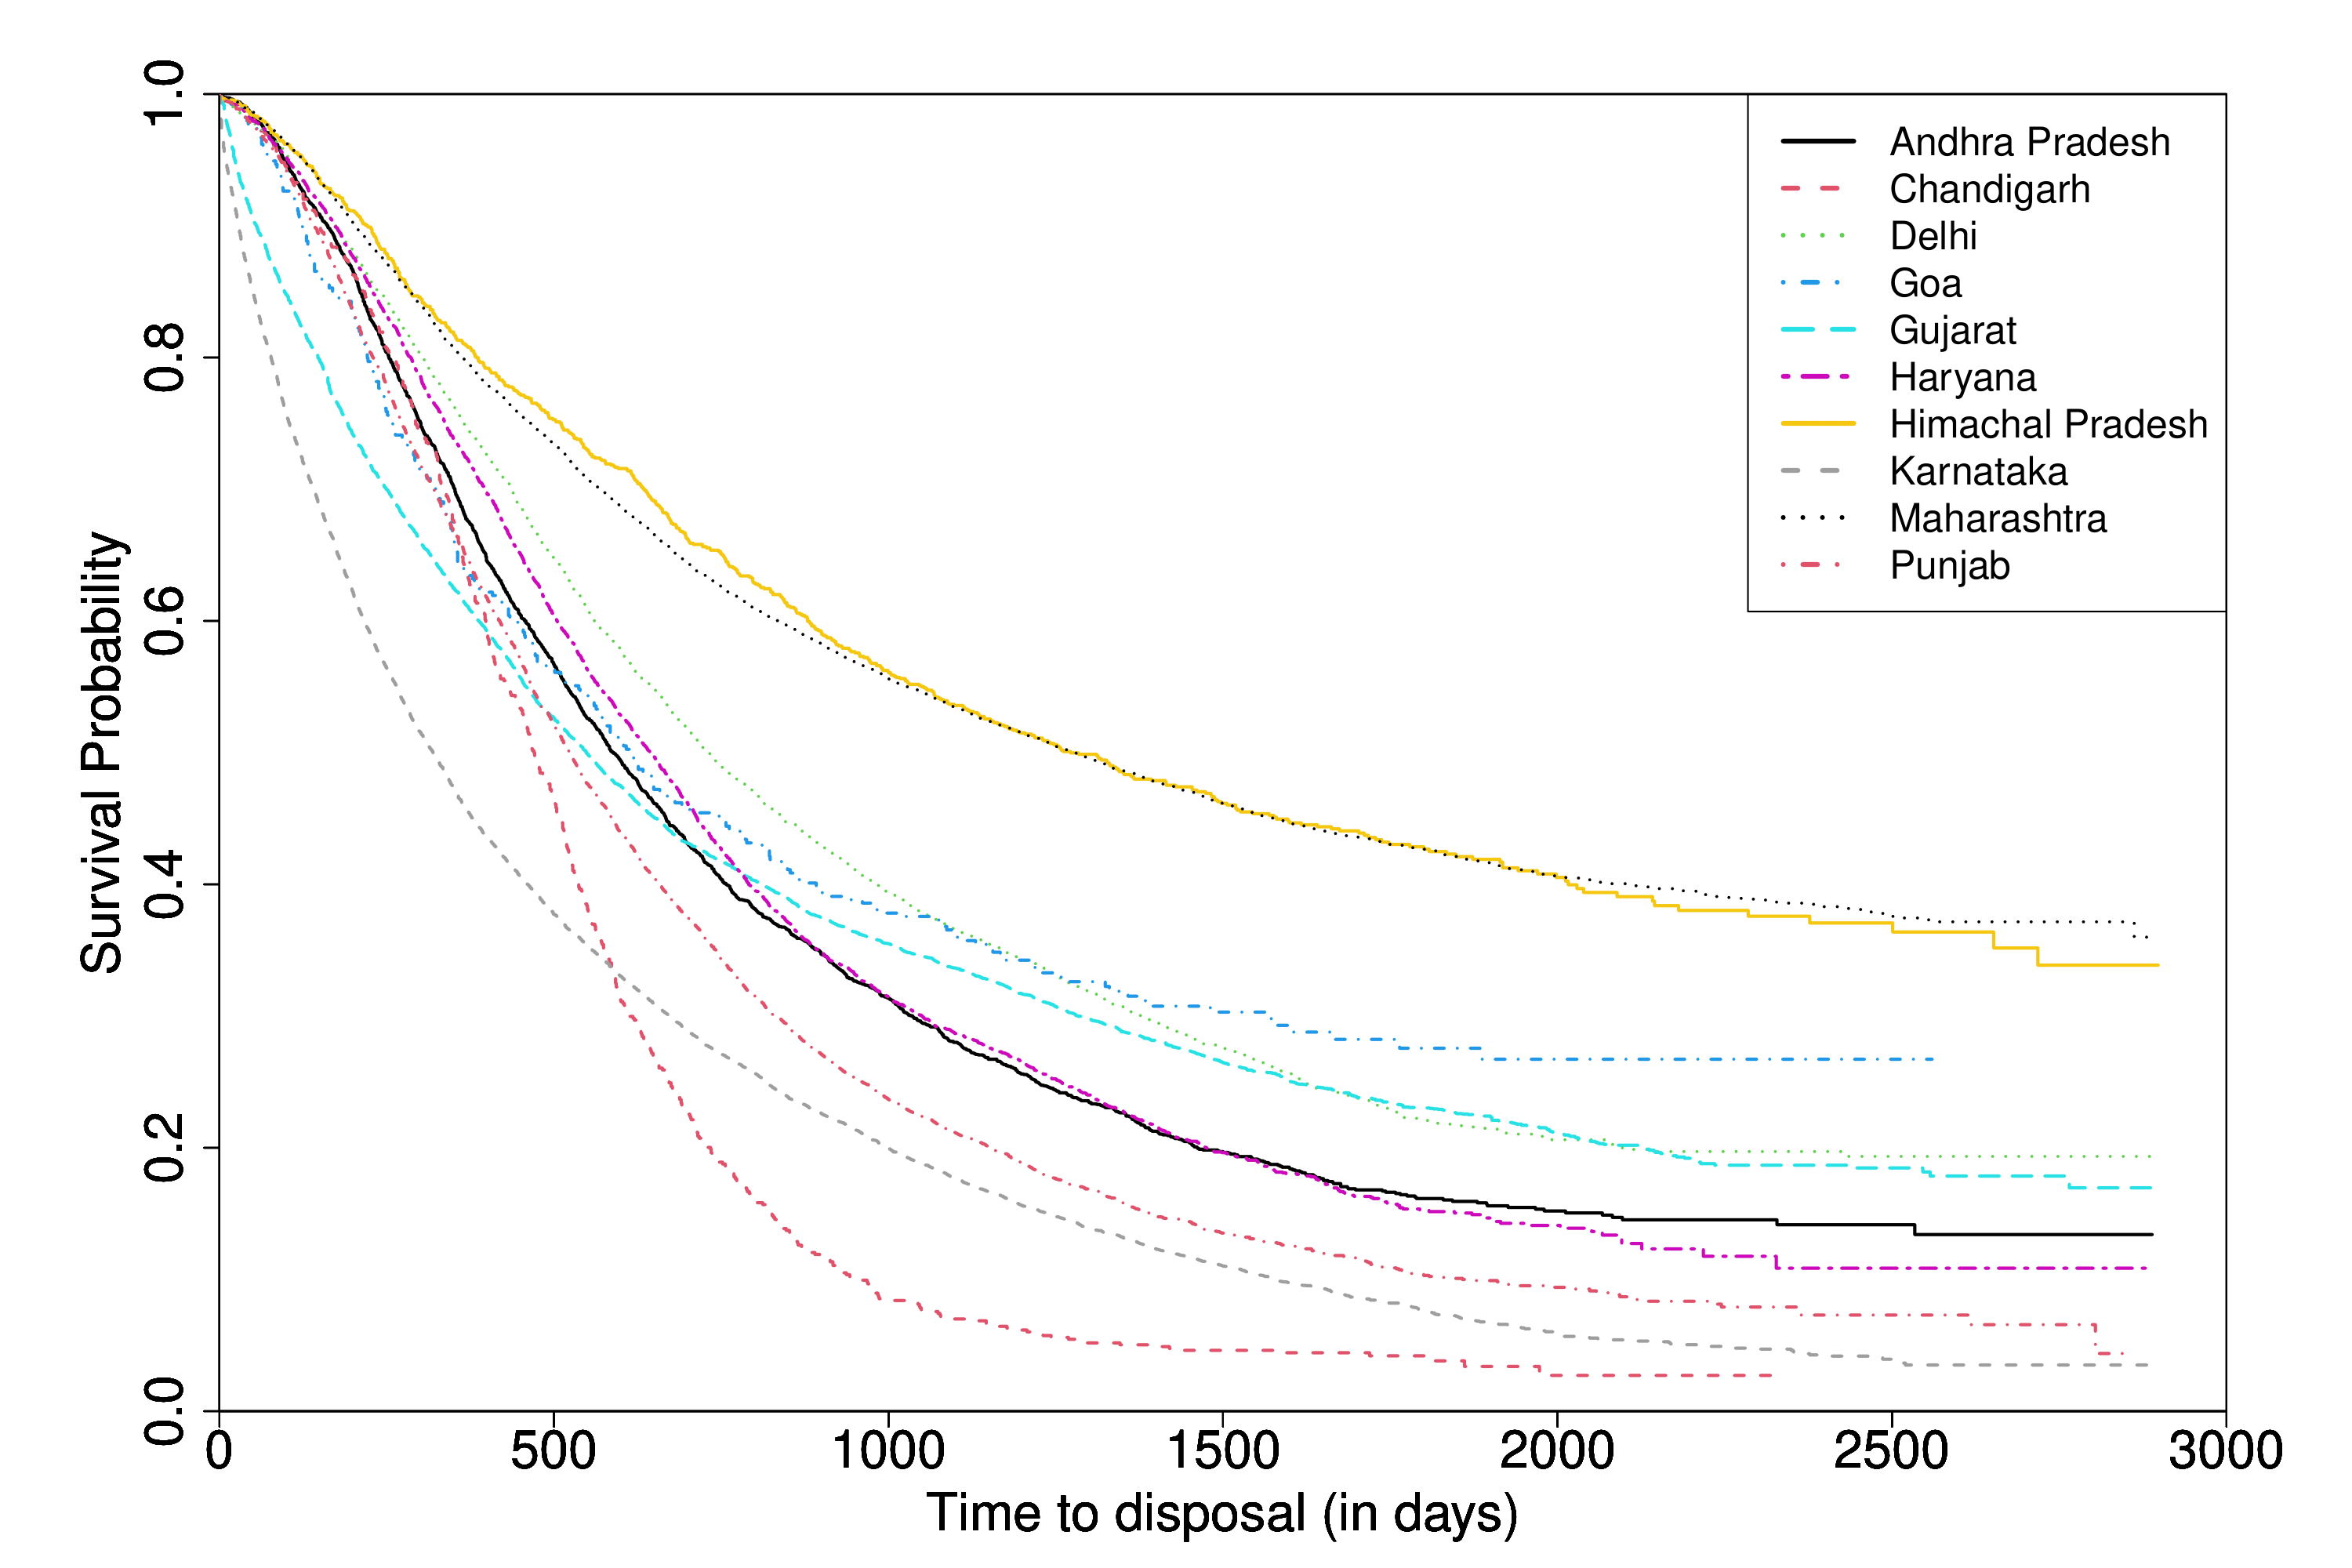
\includegraphics[width = 0.9\textwidth]{surv_states-1.png}
\end{figure}

\begin{figure}[h]
 \centering
 \caption{Survival probability of cases across years}\label{fig:yearSurvival}
 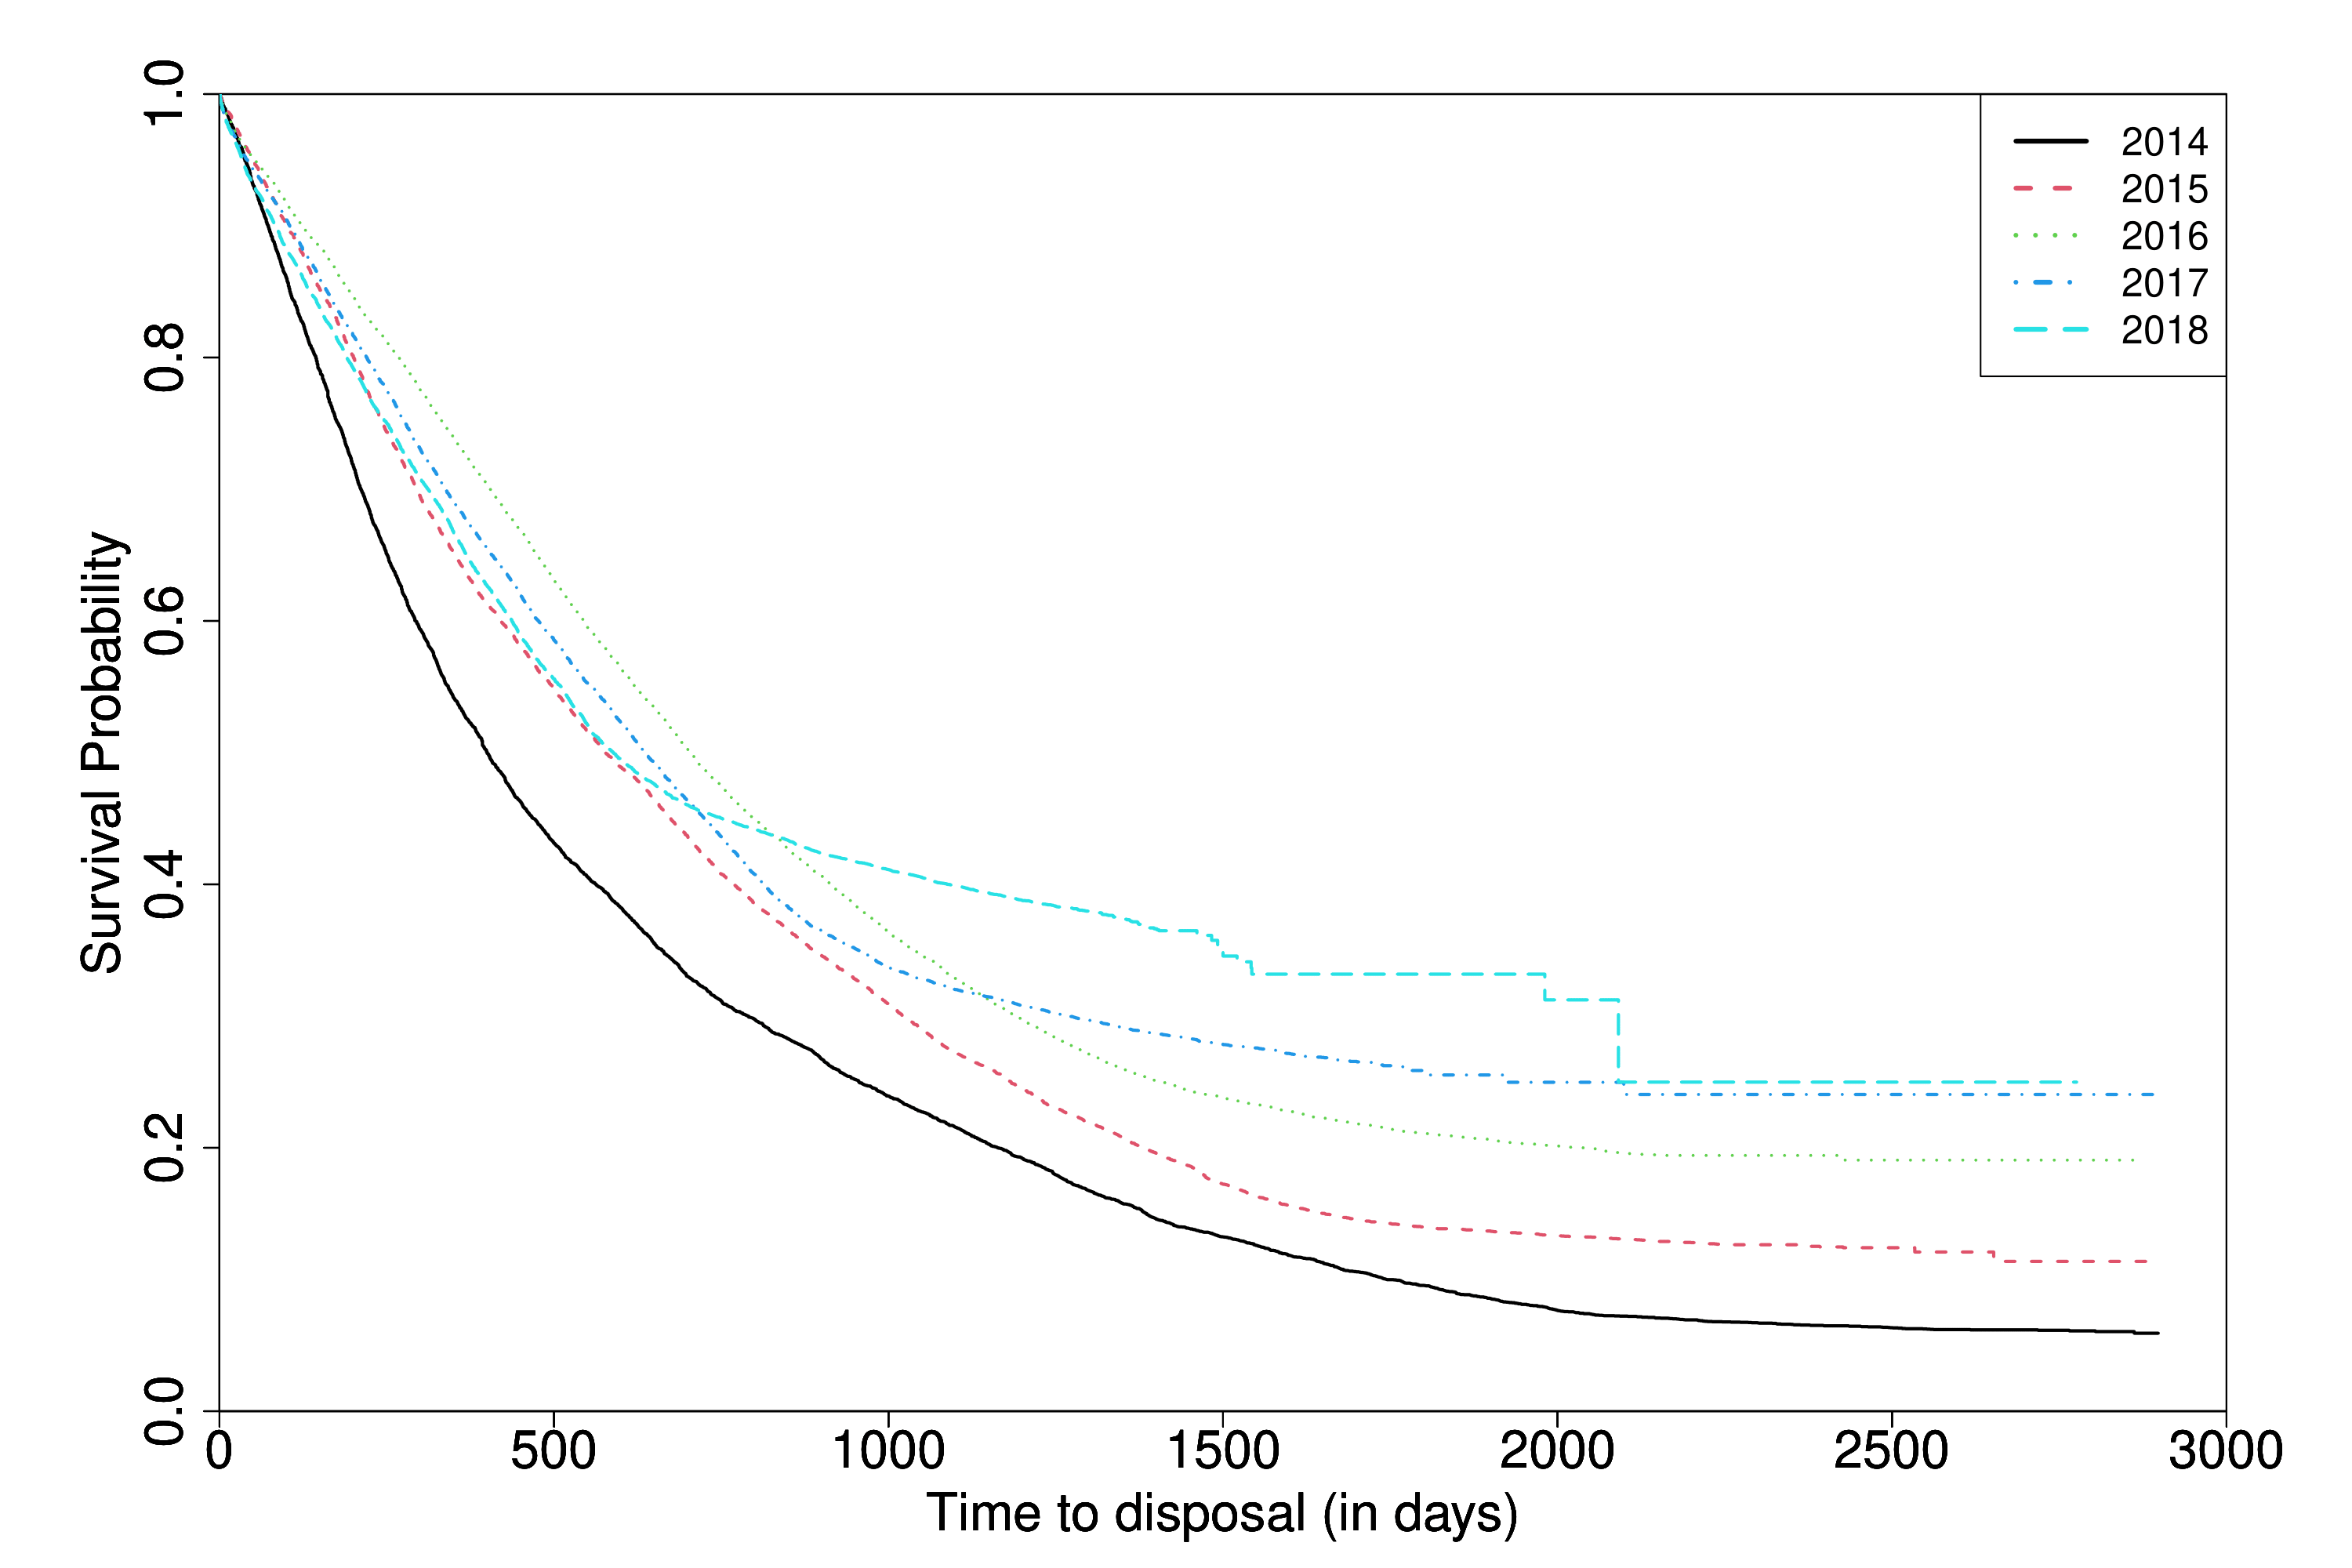
\includegraphics[width = 0.9\textwidth]{surv_years-1.png}
\end{figure}

Next, we estimate the effect of each case characteristic on the probability of the case getting disposed by the end of the observation period (i.e. 15th September 2021). Like in \textcite{datta2017_itatDelays}, we use the Cox-proportional hazard model to estimate the effect of each case characteristic. Table \ref{tab:survialProb} shows the results of the Cox-proportional hazard model. A negative coefficient indicates a lower probability of the case completing before the end of the observation period, and a positive coefficient indicates a higher probability of the case completing. As an example, jurisdictional issues and non-appearance of the accused reduce the probability of the case concluding (before 15th September 2021) by approximately 71\%, whereas the case being contested increases this probability by 55\%.

The only result that contradicts the findings of the fixed-effects model is the effect of mediation on case duration. The results of the Cox-proportional hazard model indicate that being referred to mediation increases the probability of the case concluding within the observation period by 9.7\%. However, as we have mentioned earlier, we cannot reliably identify case characteristics in pending cases. Therefore, this result has to be interpreted with some caution.

\newpage
 {\footnotesize
 \begin{longtable}[h]{lr}
 \caption{Regression result: Probability of case completion}\label{tab:survialProb}\\
 \\[-1.8ex] 
 \hline \\[-1.8ex] 
 & \multicolumn{1}{c}{\textit{Dependent variable: Probability of case completion}} \\ 
 \cline{2-2} 
 \hline \\[-1.8ex] 
			
 D(non-Appearance) & $-$0.712$^{***}$ \\ 
 & (0.013) \\ 
 D(Summons)) & $-$0.286$^{***}$ \\ 
 & (0.015) \\ 
 D(Mediation)) & 0.097$^{***}$ \\ 
 & (0.013) \\ 
 D(Jurisdiction)) & $-$0.716$^{***}$ \\ 
 & (0.013) \\ 
 D(Multiple cheques)) & $-$0.235$^{***}$ \\ 
 & (0.027) \\ 
 D(D(Contested)) & 0.553$^{***}$ \\ 
 & (0.015) \\ 
 \hline \\[-1.8ex]
 State & Y \\
 Year & Y \\ 
 \hline \\[-1.8ex]
 Observations & 46,304 \\ 
 R$^{2}$ & 0.274 \\ 
 Max. Possible R$^{2}$ & 1.000 \\ 
 Log Likelihood & $-$353,508.100 \\ 
 Wald Test & 14,569.790$^{***}$ (df = 19) \\ 
 LR Test & 14,819.270$^{***}$ (df = 19) \\ 
 Score (Logrank) Test & 15,224.080$^{***}$ (df = 19) \\ 
 \hline 
 \hline \\[-1.8ex] 
 \textit{Note:} & \multicolumn{1}{r}{$^{*}$p$<$0.1; $^{**}$p$<$0.05; $^{***}$p$<$0.01} \\ 
 \end{longtable}}


%%% Local Variables:
%%% mode: latex
%%% TeX-master: "paper_chequeDishonour"
%%% End: